\chapter{Technology Review}
Upon understanding the requirements, the development methodology and research methodology, the next part to developing the project was to apply the research methodology to investigate what technologies we would need to use to develop our mobile application. We knew that we would using a framework coupled with a coding language. We started by looking towards the software industry itself and seen what exactly was being used at this time. From our research two frameworks stood out to us. First was Ionic, a framework that combines the core Ionic user interface components, gestures and animations while also using tooling and application programming interface's (API) which are tailored to Angular Developers. 

\section{Frameworks and languages}
Ionic\cite{Ionic} is built to work naively on both web and mobile platforms by using an open source programming language known as TypeScript. This language is used to build large scale applications (e.g. Slack, DoorDash and BitPanda). The reason for this is Ionic uses Angular (a development platform) which was built with TypeScript. Interestingly, TypeScript is a typed super-set of JavaScript meaning that any code typed in TypeScript would just compile into plain JavaScript\cite{tsIntoJS}. Despite this, to develop Tipper in Ionic with TypeScript, we would have to learn TypeScript. We understood this and had to weigh up the benefits of this. As mentioned previously, the purpose for choosing a project like this was to learn a language and framework used widely in industry. 

The other framework we wanted to look into was React-Native, a platform specific open source user interface framework. It is touted as a framework that is used by developers of all skill levels with their documentation intended to be easy to understand by following a clear step by step tutorial style. Over the course of our research, we learned that React-Native was developed by Meta (formerly Facebook)\cite{reactnative} and was originally considered developed enough to be used native applications, but it seems that times have changed. It has been used by Meta owned companies (Facebook and Instagram) and other major tech companies such as Discord, Skype (owned by Microsoft) and even Tesla\cite{reactnative}.


When a new React-Native project is created, the language it is built with defaults to TypeScript but JavaScript can also be used. For example, if we created a .js file, (which stands for JavaScript) its interpreted as a JavaScript file and will not type checked. Then files with a .jsx extension are treated as JavaScript instead of TypeScript. JavaScript is a scripting/programming language that would allow us to implement complex features into our application. We had some experience with this language which we feel it definitely had an impact on our choice for a framework to develop our application with. 


We also wanted see the adoption rate of both languages, where is it being used and more specifically, which is used more in industry. Statista conducted a survey from May 11 to June 1, 2022 where 71,547 respondents answered the question of what language do they use. The results showed that JavaScript held a huge majority of 65.36\cite{mostused} percent where as TypeScript held 34.83\cite{mostused}  percent share. Interestingly, HTML/CSS held 55.08\cite{mostused}  percent of developers saying that the use. From our work on the app so far, we know the HTML/CSS isn't necessarily used on for mobile application development but is similar. It uses style sheets and tags for the user interface. We have included an image of the top ten languages below. 

\begin{figure}[h]
  \centering
  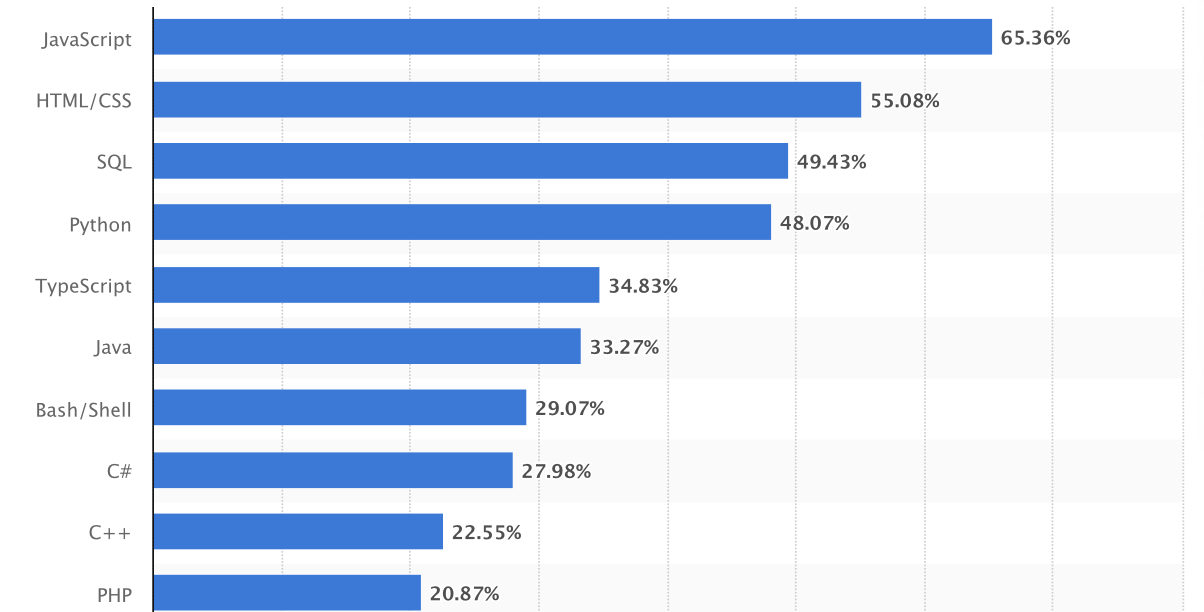
\includegraphics[scale=.65]{atu-computing-latex-template/images/top10Languages.png}
  \caption{List of top 10 programming languages in 2022}
  \label{fig:top10languages}
\end{figure}
It was very important to look at the components that each framework offered within their respective libraries. We understood that we had some requirements to make this application work. When looking at how we would connect the two users, quick response\cite{soon2008qr} codes stood out to us, as they were unique to each individual user. We noted that other applications use them such as Snapchat. How it works on that platform is when a user creates an account they are given a unique QR code which can be accessed from their account page and can be scanned by another user to send a friend request without having to enter a username or phone number. We tested that option and noticed how seamless it was. It seemed to fit our requirement, helped to protect peoples information (an example is not handing out a phone number). Prior to starting this project, we didn't know that QR codes were just a visual representation of text such as a website or a username. \cite{soon2008qr}

We came to the conclusion that React-Native, coupled with JavaScript would be the best option for us as it would be worth learning this language and framework. The statistics tell us that there is a reason JavaScript is so widely used in industry. As we already mentioned already we had some previous experience with JavaScript and to a lesser extent TypeScript, but having to learn an entirely new language to us could cause problems that we would have liked to avoid. In addition, when doing our research to make our decision we noted that the number of resources for React-Native JavaScript development seemed to be greater as opposed to Ionic/TypeScript development. It's is also worth noting that some packages that would be vital to developing this project were easily find-able with a Google search whereas Ionic, not so much. So in the end React-Native with JavaScript was our clear choice. 
\section{Packages}
At the start, we thought that we would need to source a third-party software or a website to do this. The question then was, how do we implement them into our project. Then we came across two packages built into React-Native that could be installed. The first we learned about was react-native-qrcode-svg. This package had the ability to generate a QR code with information that was input by the user\cite{npmQrSvg}. This package did require another dependency though, that being react-native-svg. The purpose of this package was to add svg support to the project\cite{npmSvg}. To add install these packages, you need to run the command either 'npm i react-native-svg' and then 'npm i react-native-qrcode-generator'. NPM was the choice of package manager that we chose to use but more on package managers later. Our reason for choosing a QR code system is that we noticed that restaurants have generally have QR codes inside to bring the user to a web page to view the menu. 

SVG, which is short for Scalable Vector Graphic\cite{cagle2008svg}, is unique type of image format. SVG's doesn't rely on unique pixels to draw it's images but rather uses Vector data which is just an element with a specific magnitude and direction\cite{cagle2008svg}. This type of format makes it a perfect choice for drawing QR codes within our application. You can also have Portable Network Graphic's (PNG's) for a QR code but isn't suitable for the our purposes because if you need to resize a PNG QR code, the image becomes distorted which can result in potential data loss from a generated QR code. We learned that PNG codes are more widely used in industry but we were not able to find any packages on React-Natives website that would allow us to generate PNG QR codes so despite the pros and cons of both, we had no choice but to use SVG generated QR codes. 

The QR code generation library allows the user enter some values to change some aspects to the code that is generated. Most importantly we are able to adjust the size of the QR code on the screen, the color and the background colour which allows for personalizing. We noticed that we would also need a way for the user to be able to save their generated QR code. There is two ways we wanted to go about this. The first was to just save it to the users camera roll via a save button. We learned that there is another package that we could use named 'react-native-fs'\cite{rnfs} with fs meaning File System. To import this package we would run the command 'npm i react-native-fs'. With this command we realised that the user would have a way of saving a QR code without having to take screenshots and then the user having to adjust the size of the screenshot. With this though, the user has to give permission for our application to write the image to their camera roll. 

The other way we wanted to allow the user to have the QR code was to have a button that would send an email with the QR code to the email address that was used to when the user signs up. React-Native has a package to solve this issue we faced named 'react-native-email\cite{npmEmail}'. To install this package we would have to run the command 'npm i react-native-email'. With this package, we would be able to have a email address where the QR code would be sent to, and would also allow us to edit the carbon copy, blind carbon copy, subject and finally the contents of the email itself. With this the user has a way of saving the QR code that they generated locally on their device and also a copy saved to their email address. 

For this application to work, we would need a way for the user to scan a QR code. We again looked at the Snapchat example, which heavily uses the camera on a device as one of its main features. It made sense that we would be doing the same because a QR code is pointless if it cannot be scanned. Once again, React-Native had a library for this, aptly named 'react-native-qrcode-scanner'. Similar to the other packages mentioned, to install this package we had to run the 'expo i Barcode-Scanner' command\cite{barCodeScaner}.

The documentation for the packages Barcode-Scanner and react-native-fs mentions that on iOS devices running iOS 10 or earlier needs to have some code added to info.plist, a file in the iOS folder of the project. We learned that iOS 10 is no longer supported on the App Store (the app for downloading apps on iPhone) so even if this application would put on the App Store, devices running iOS 10 cant even download apps. Since October 2022, only devices running iOS 12 and on-wards can download apps. The latest version of iOS is 16 so there is no chance of this becoming an issue. The reason for this is we needed a way to give permission to user to be able to allow the app to use the camera. 

For this project, we need a way to navigate around the app, say for example when we press a button or an event happens. The React-Native library has a package for this as well named 'react-native-navigation'. This provides 100 percent native platform navigation on both iOS and Android\cite{npmNavigation}. Like the other packages thus far, its installed with 'npm i react-native-navigation'. There really isn't too much to say about this package. You just have to add a Navigation tag into the app.js and import an index.js file that with the different screens which allows the user to move to different screens in a stack format. Each page is rendered on top of another allowing us to go back forth with ease. 

\section{Devices we are developing for}
When developing a mobile application, we need a way to be able to see how the front end looks when we make a change to it. We needed to learn how we would go about that. First we found out what mobile devices we would have access to. We had an iPhone 14 Pro Max and would be developing the application on MacOS Monterey 12.6. We looked into obtaining an Android device but that was not possible. We learned that both Apple and Google offered simulators that would run on our machine but for both platforms, this required some setup to get this to work. Prior to realizing, getting an Android device was not possible, we did find out how we would go about that.

For Android, we would have needed to install Android studio\cite{meetAndroidStudio} the official Integrated Development Environment (IDE) for Android app development. Even though this is a code editor, we wouldn't actually use this to write our code (we used Visual Studio Code but we will discuss that later) and just needed to get the Android Emulator. From the documentation we learned that you would install the emulator through Android Studio by choosing the Android version we would like to develop for\cite{installAndroidStudio}. We also needed NodeJS, an open source server environment for running the application. After setting up Android Studio, we would have needed to create a React-Native application within a folder in the terminal with the command 'create-react-native-app Tipper', select which platform we would be developing for. Finally when that was all done, run the command 'npm run android'. Below is an example of what this may look like. Also Yarn is a package manager like NPM. We used NPM for this project.
\begin{figure}[h]
  \centering
  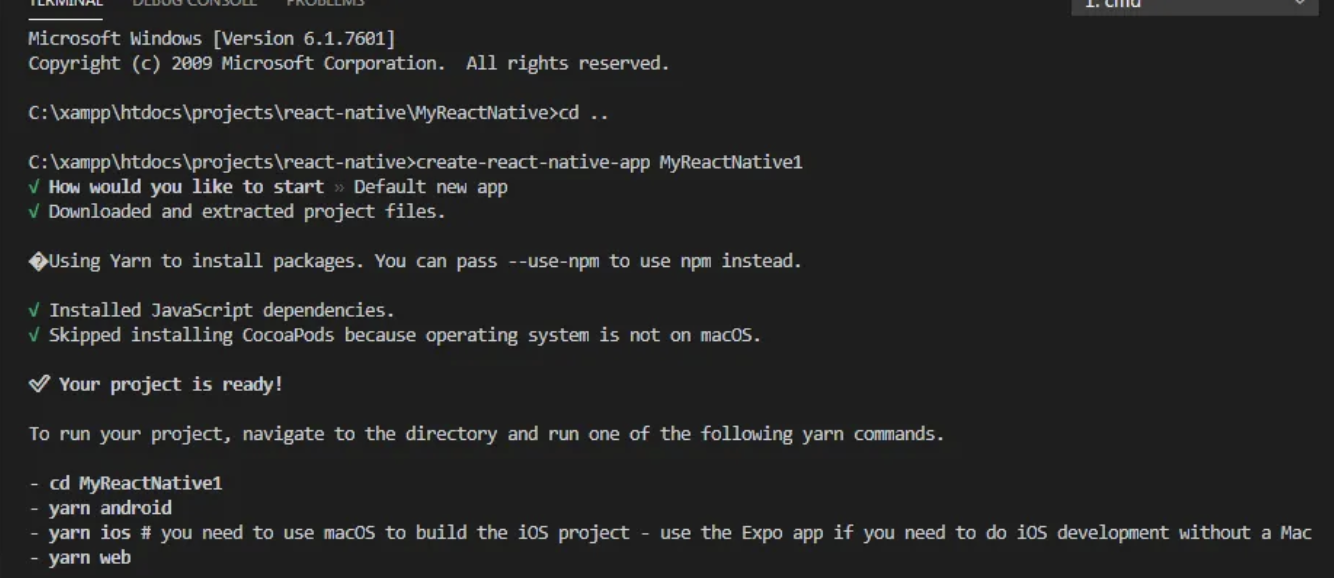
\includegraphics[scale=.55]{atu-computing-latex-template/images/Screenshot 2023-04-18 at 19.08.30.png}
  \caption{Setting up a react-native project}
  \label{fig:{Setting up a react-native project}}
\end{figure}
And by running the command 'npm run android', we would see something similar to this. 
\begin{figure}[h]
  \centering
  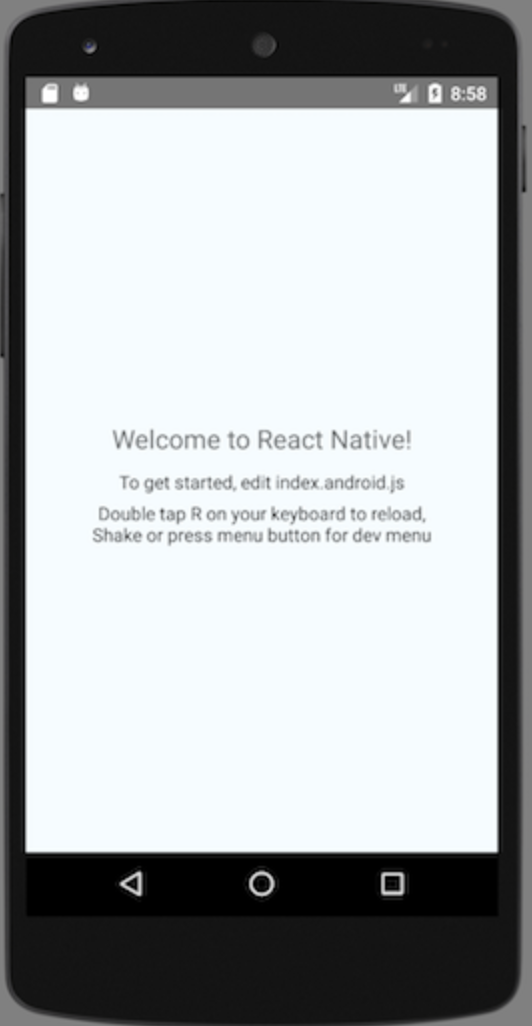
\includegraphics[scale=.55]{atu-computing-latex-template/images/Screenshot 2023-04-18 at 19.13.37.png}
  \caption{Android Emulator running}
  \label{fig:{Android Emulator running}}
\end{figure}
\section{Setting up the development environment}
The process setting up an iOS simulator is quite similar but we learned that there were some caveats for this. Firstly, like developing for Android which requires Android Studio, you need to download XCode, Apple's integrated development environment for MacOS and MacOS only unlike Android Studio, can be installed on Windows, MacOS, Linux and Chrome OS. Written in C, XCode is touted as being much faster with a twenty-five percent increase in project build speed with the latest version (that being XCode 14)\cite{XCode} and with "simplicity and power of Swift and SwiftUI with a new multiplatform app experience". Then when looking at forums and discussions about XCode where we observed multiple threads about XCode's poor performance, crashes and unusual errors. 

We have to admit this did become a cause for concern. We were building this application on a base model, 2019 MacBook Pro with 1.4 GHz Quad-Core Intel Core i5 CPU and 8GB of 2133 MHz LPDDR3 Random Access Memory and 256 Gigabyte Solid-State Drive. We also noticed that users who had an improved performance experience of XCode were running Mac's with Apple's in-house built Sillicon chips where as our machines were running Intel chips. The size of XCode to install was around 11.7 Gigabytes but required the install device to have around 40 Gigabytes free on disk. That wasn't even the end of it. The more versions of iOS and Simulators we installed, the install size grew fast. The reason for the massive size is the fact that XCode supports MacOS(Desktop/Laptop), iOS(iPhone), iPadOS(iPad tablets) and TvOS(Apple TV's). Then on top of that, each device having multiple versions of their operating systems having different simulator runtimes, libraries, compilers, and software development kits.

When it came to setting up the simulator for the iOS devices on our machine, we had to jump through a few more hoops. First of all we needed a package manager. We had three options for doing this. The first was Node Package Manager or NPM. The second was Yet Another Resource Negotiator or Yarn and finally Homebrew. They all essentially did the same thing. Homebrew was only available on MacOS. NPM was the package manager that we had previous experience with and Yarn we never used before. The main difference between NPM and Yarn is NPM installs packages sequentially where Yarn installs dependencies in parallel. A smaller difference was when installing a package, was simply if you said either npm install or yarn add. Although to install NPM or Yarn on MacOS, we would have needed to use Homebrew. 

The next step we needed to do was install Node.js\cite{setUpDevEnviro}. Upon doing this we we realised that Node.js was already installed on our machine from working on previous projects. How we knew this was running the command 'node -v' in the Terminal. If it was a case that we didn't have it installed, we would have needed to download from the install file from the Node.js website.

Next we installed Watchman, a piece of software that detected changes to code and refreshed the simulator to show this\cite{setUpDevEnviro}. Say if we changed the colour of a button in our application, the simulator automatically refreshed and was displayed to us. Next we needed XCode installed on our machine which we got from the App Store. Upon installation, we installed a simulator by selecting the iOS version we wanted in the components settings. Next was install Ruby (which was also already on our machine) and Cocoapods. The reason for this, when we would install a package, we needed to link the package to the iOS device, also known as Pods\cite{setUpDevEnviro}.

Finally, we created the React-Native project using it's Command Line Interface(CLI)\cite{setUpDevEnviro} with the command 'npm react-native@latest init Tipper'. This generated our project and all of the files that we would need to start development. Then to run the iOS simulator we ran the command (from the projects root directory) 'react-native run-ios'. This will open the XCode simulator\cite{iOSSimulator} and start to build the project. Initially we found the build process painfully slow. We later discovered that the reason for this was the folder was stored on iCloud Drive, Apple's cloud storage solution and was trying to sync everything over the internet which killed our performance. What we saw was nearly identical to running the Android Emulator but showed an iPhone instead of an Android device.

For the Integrated Development Environment (IDE), we chose to use Visual Studio Code which is a rich-text editor. A lightweight code editor that runs on MacOS, Linux and Windows\cite{VSCode}. When it came to choosing an IDE, we wanted to use something that is reliable and easy to use. We were very familiar with Visual Studio Code from working on previous projects over the course of our education. That isn't to say that we didn't at least explore other options. As mentioned before XCode was an option that we could have used but because of the reasons mentioned before, we chose not to go with that.

Visual Studio Code also offers customisable features in the form of plugins for developers to curate a pretty selective development environment. Along with built-in support for Node.js, TypeScript, and JavaScript, it quickly stood out to us as a choice for developing our project with.

Next we decided to look at Android Studio. We looked at what it had to offer but quickly decided against this. Mainly because that Android Studio is used primarily for development on Android devices\cite{meetAndroidStudio} which we would not have access to any devices to properly test outside of the simulator. This was important because the package 'react-native-qrcode-scanner'\cite{npmQrSvg}, which scans the QR code using the camera, will only work on physical devices and not on Android's emulator or XCode's simulator. We would need access to a camera and neither can provide this. 

Finally we looked at Visual Studio, the 'big brother' to visual studio code (both are Microsoft products). This is an actual Integrated Development Environment which offers features such as editing, debugging capabilities, code completion tools, compilers and graphic designers\cite{VS}. Visual Studio can come in a free and paid version as opposed to Visual Studio Code which is free regardless. Both also have their own benefits and drawbacks. Visual Studio's performance is noticeably slower (we have first hand experience of this) where as Visual Studio Code's IntelliSense (Code auto-completion) is worse. The one thing that stood out to us was the install size difference between the two. Visual Studio Code uses around 500 Megabyte\cite{VSCode} where as Visual Studio can take anywhere between 2.3 Gigabyte and 60 Gigabytes\cite{VS}.

When we took everything into account between performance speeds, install sizes and the features that is offered, Visual Studio Code was the clear choice to develop our project with. We can speak from first hand experience that Visual Studio is slower in comparison to Visual Studio Code, XCode's performance was also not favourable on our machine and Android Studio did not meet the requirements the decision we felt was not difficult to make. 
\section{Choosing a database}
The next technology that we needed to make a decision on was the database we would use to store our information. We knew that this would primarily be used for storing login information and maybe some smaller pieces of data, e.g. a users QR code. At the start we thought that MongoDB would be a good choice. MongoDB is a document database\cite{mongodb} that could be used at any scale. The data is stored in JSON like objects and used multiple massive tech companies such as Google, eBay and Electronic Arts. Before also making the decision on how we would store payments, we learned that MongoDB recently started supporting multi-document transactions. These are atomic (meaning all-or-nothing)\cite{mongodbTransaction}. So if a transaction commits, the data changes made in the transaction are not visible outside the transaction.

We soon learned of third-party services that would handle the transactions that being Stripe (discussed below) and other databases that would handle the login/security features and resetting of passwords using built in methods. This seemed like a good idea to use. Another reason for this is we learned that MongoDB was more suitable for desktop applications in comparison to mobile applications. The option that stood out to us was AWS Amplify, a database solution that is owned by Amazon and is apart of Amazon Web Services that lets front-end web and mobile developers easily build, ship, and host full-stack applications on AWS. Setting up Amplify seemed quite straight forward. The documentation said that all we would need to do is a few steps. The first was to install AWS Amplify CLI, then setup a database and set the data models used signing up and for authentication\cite{amplify}. 

When you hit deploy at the bottom of the page, you are presented with a command that is unique for your database. Run that command in the root folder of the project. Finally copy the configuration code also presented with the command into a config.js file. From there you have access to methods such as 'signUp()', 'forgotPassword()' and 'signOut()' by adding import Auth from 'aws-amplfy' . Overall it seemed straight forward enough. The documentation was thorough and detailed. AWS also had videos showing us how to get this setup. 

Amplify offers other features such as push notifications, Artificial Intelligence and Machine Learning predictions, different data storage solutions and REST API's. Amplify proved to be a robust choice for our back-end that would allow us to expand the project in multiple ways if so we chose too while also satisfying our needs for what we needed at the moment\cite{amplifyFeatures}.
\section{Transactions}
Finally, we needed to decide on the way we would process payments from one user to another. First we thought about using Apple Pay but soon decided against this. Implementing Apple Pay required us to sign-up for an Apple Developer account, a merchant identifier along with other hoops to jump through\cite{ApplePaySettingUp}. We also didn't want this application to become Apple dependent. We were already developing on MacOS, XCode and for iOS. We felt it would be best to try and incorporate as many unique technologies as possible. That is when we came across Stripe, an Irish-American company that on their website, says works with startups to large enterprises. We seen that they offered solutions for everything we needed and more. We admit that we were skeptical as we never worked with something like this before (money and security) so we had to base everything we knew off of online discussions and what was on Stripes website\cite{stripe}. From what we learned implementing Stripe would be far easier and meant that we were not tied to Apple Pay. This also meant that we could expand to other platforms easier. We knew that we would need to use ExpressJS(back end web application framework for building RESTful API's) and Node (Node.js is a back-end JavaScript runtime environment) because to connect to Stripe, we need a simple server that can contact Stripes servers to start a transaction when they payment flow is called. Stripe is implemented using a 'Secret Key' to connect to our Stripe dashboard and a public key that is called when a transaction is going to be made.